\documentclass[12pt]{article}
\usepackage[left=1in, right=1in, top=1in,bottom = 1in]{geometry}
\usepackage{amsmath}
\usepackage{xcolor}
\usepackage{lmodern}
\usepackage{listings}
\usepackage{graphicx}
\usepackage{float}

\lstset{language=[90]Fortran,
  basicstyle=\ttfamily,
  keywordstyle=\color{red},
  commentstyle=\color{blue},
  showstringspaces=false,
  morecomment=[l]{!\ }% Comment only with space after !
}

\begin{document}
	\begin{flushleft}
		Max Le \\
		ID: 901223283\\
		MTH 5050: Parallel Process\\
        Assignment 4: Applications of OMP on Collatz Conjecture
    
	\end{flushleft}

        
        
        \section{Introduction}
            In this assignment, the goal is to parallelize a code that follows the Collantz conjecture. The conjecture states that starting with any integer n: 

            \begin{itemize}
                \item if n is even, then n = n/2
                \item else if n is odd, then n = 3n + 1 
            \end{itemize}
            
            This sequence then continues and according to the conjecture, all cycle will eventually terminates at 1. \\
            For the current assignment, we are going to perform this procedure on a range of numbers, then for each of the number, we are going to try to record the highest n ever reached per range of numbers. \\
            Our given range of numbers to be used are from 1 up to 2,000, 20,000, 200,000 and 2,000,000. \\
            The problems are to be completed using OMP and different parallel schedules are experimented.  

        \section{Approach}
            For this problem, the algorithm for Collantz is relatively simple. Below is the snippet of the subroutine for this conjecture:
            \begin{lstlisting}
        SUBROUTINE hotpo(ndum)
            IMPLICIT NONE
            INTEGER*8, INTENT(INOUT) :: ndum

            IF (mod(ndum,2) == 0) THEN
                ndum = ndum / 2 
            ELSE
                ndum = (3 * ndum ) + 1
            END IF

            IF (ndum == 1) THEN
                ndum=1
            END IF
        END SUBROUTINE hotpo                
            \end{lstlisting}
        \newpage
        \noindent
        Then, the challenge is to decide which OMP schedulers is appropriate, as well as which variables to be made private and share.  In this code, the loop variables and local max number are chosen to be private, while the start and end loop variables are shared.  The tricky part would be to determine the global max,this is done via the reduction clause so that we can find the maximum over all threads. In code, it looks something like this:

        \begin{lstlisting}
!$OMP PARALLEL DO SCHEDULE(GUIDED,4) PRIVATE(iterNMAX,j,n,highN)&
!$OMP SHARED(maxHOTPO,nstart,nend) REDUCTION(max:GLOBAL_MAX) 
DO iterNMAX = nstart,nend
    n = iterNMAX
    highN = 0
    DO j = 1,maxHOTPO         
        !! local max 
        IF(n > highN) THEN 
            highN = n 
        END IF
        
        !! calling hotpo subroutine 
        call hotpo(n)

        IF (n == 1) THEN 
            EXIT 
        END IF
        !! global max 
        IF(highN > GLOBAL_MAX) THEN 
            GLOBAL_MAX = highN
        END IF
    END DO
END DO
!$OMP END PARALLEL DO 
        
        \end{lstlisting}                

        In terms of the schedulers, different types of schedulers will be investigated.  These include: static, dynamics and guided. Additionally, chunk sizes are also investigated.  For simplicity, chunk sizes of 1,2,3 and 4 are experimented for a specific number of thread: 4.  This was chosen because 4 threads give steady performance across different problem sizes and scedulers.   
    
        \newpage
        \section{Results}
        \subsection{Maximum N }
        Firstly, below are the problem size the corresponding maximum N:

        \begin{center}	
            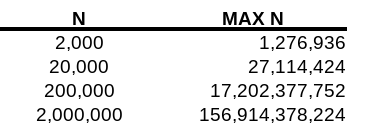
\includegraphics[width = 80mm,height = 25mm]{result_max.png}
        \end{center}
    
        \subsection{Default Schedulers}
        Below are the results when using default schedulers: 

        \begin{center}	
            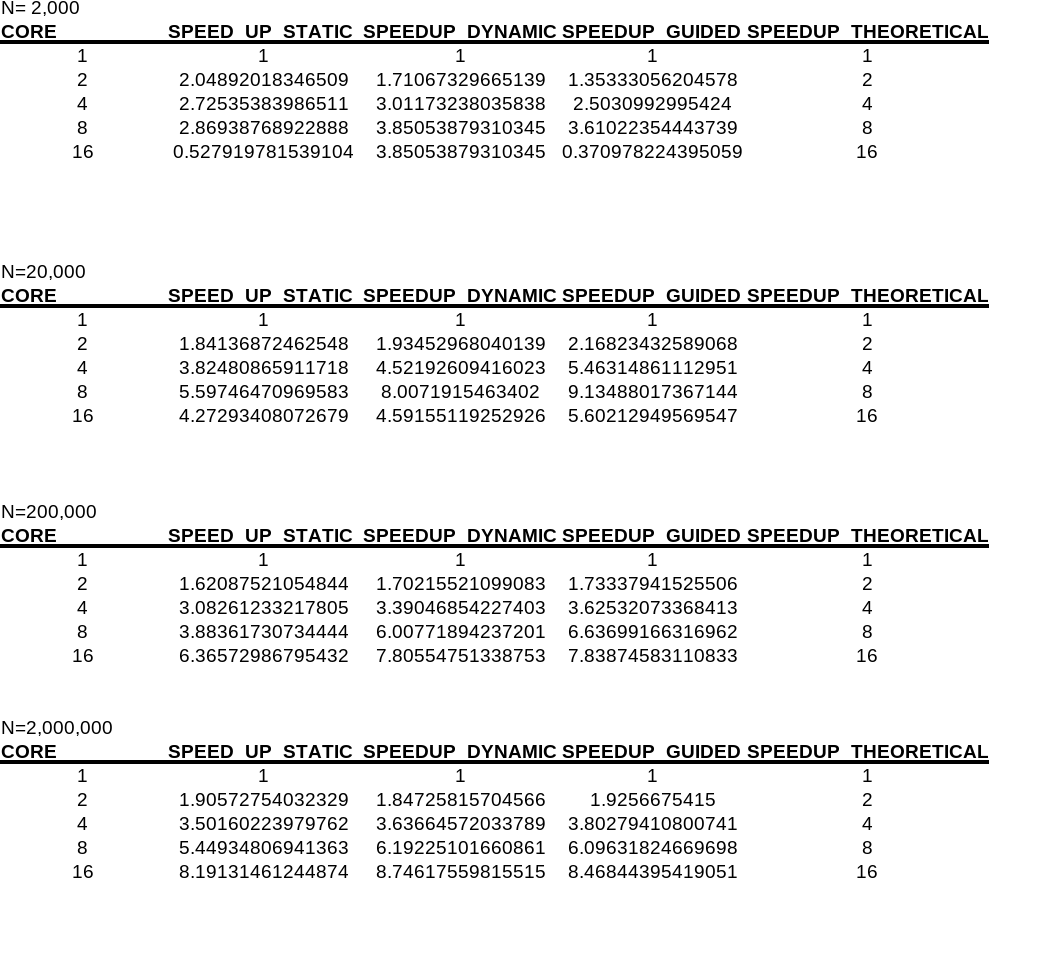
\includegraphics[width = 150mm,height = 150mm]{result_speed.png}
        \end{center}

        \newpage
        In order to make it easier to visualize, the plots for the above data are produced per problem size as follow: 

        \begin{figure}[H]
            \hfill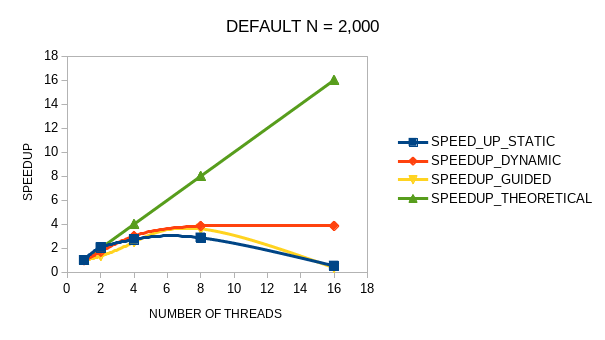
\includegraphics[width=150mm,height= 80mm]{speedup_2e3.png}\hspace*{\fill}
            \caption{Default schedulers for N = 2,000}
        \end{figure}        


        \begin{figure}[H]
            \hfill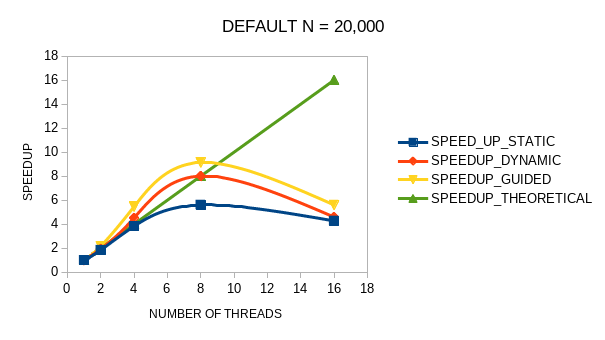
\includegraphics[width=150mm,height= 80mm]{speedup_2e4.png}\hspace*{\fill}
            \caption{Default schedulers for N = 20,000}
        \end{figure}        

        \begin{figure}[H]
            \hfill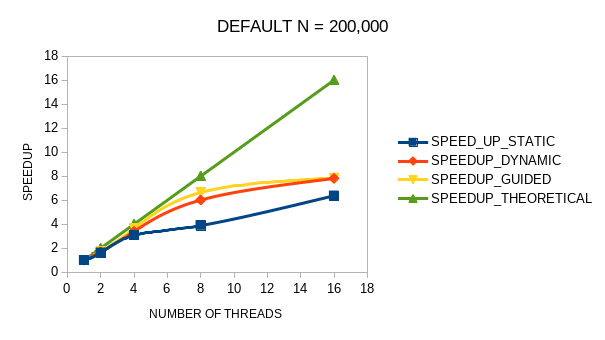
\includegraphics[width=150mm,height= 80mm]{speedup_2e5.png}\hspace*{\fill}
            \caption{Default schedulers for N = 200,000}
        \end{figure}        

        \begin{figure}[H]
            \hfill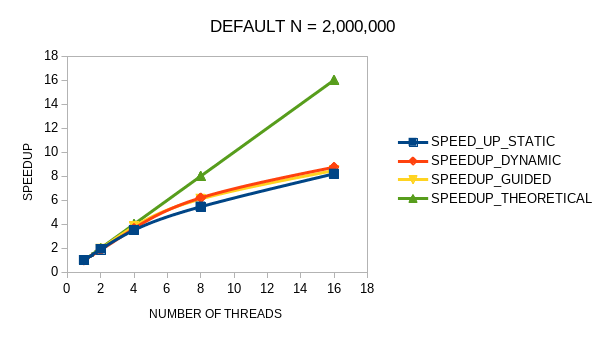
\includegraphics[width=150mm,height= 80mm]{speedup_2e6.png}\hspace*{\fill}
            \caption{Default schedulers for N = 2,000,000}
        \end{figure}        
        \newpage
        \subsection{Chunk Sizes}

        \begin{center}	
            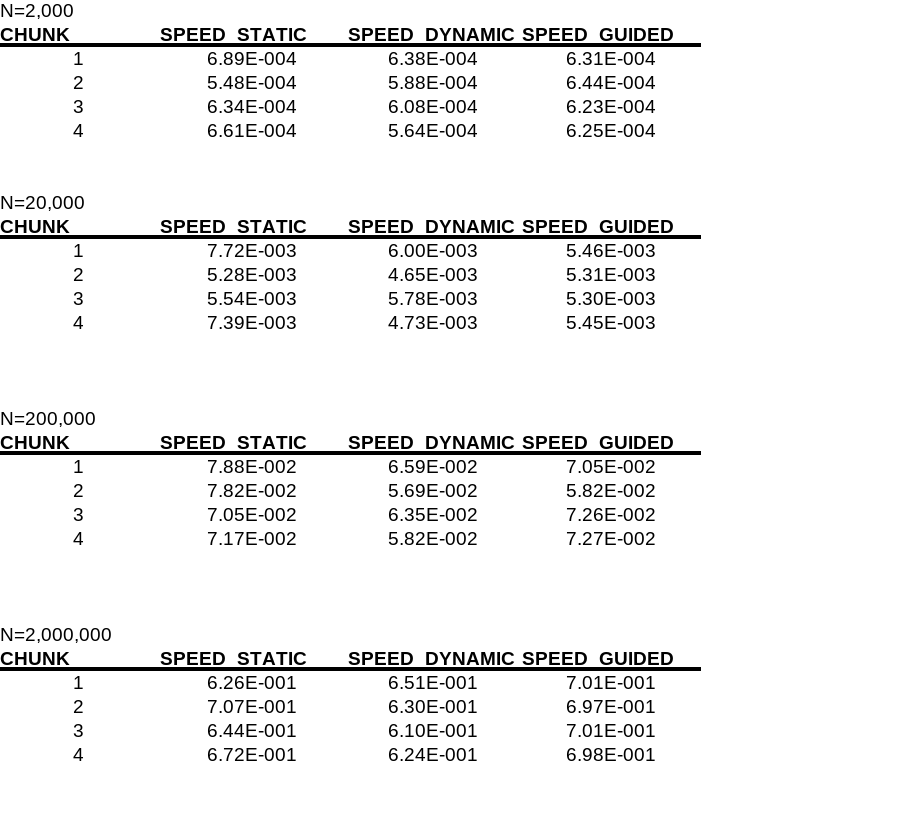
\includegraphics[width = 120mm,height = 120mm]{result_chunk.png}
        \end{center}

        Below are plots of chunk size vs. different speed from different schedulers. 

        \begin{figure}[H]
            \hfill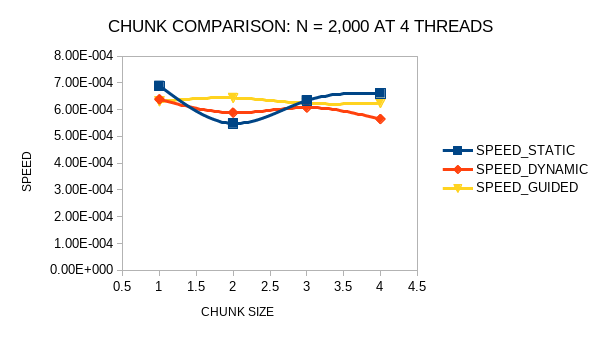
\includegraphics[width=150mm,height= 80mm]{chunk_2e3.png}\hspace*{\fill}
            \caption{Chunk size comparison for N = 2,000}
        \end{figure}  

        \begin{figure}[H]
            \hfill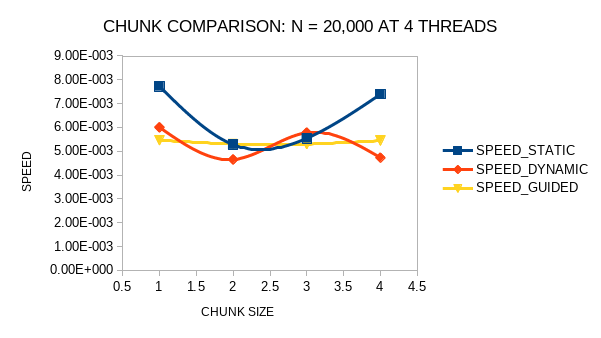
\includegraphics[width=150mm,height= 80mm]{chunk_2e4.png}\hspace*{\fill}
            \caption{Chunk size comparison for N = 20,000}
        \end{figure}  

        \begin{figure}[H]
            \hfill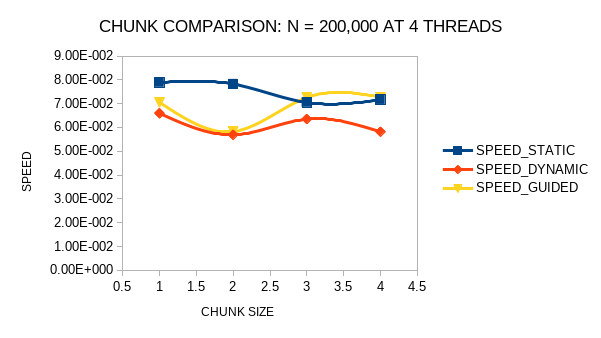
\includegraphics[width=150mm,height= 80mm]{chunk_2e5.png}\hspace*{\fill}
            \caption{Chunk size comparison for N = 200,000}
        \end{figure}  

        \begin{figure}[H]
            \hfill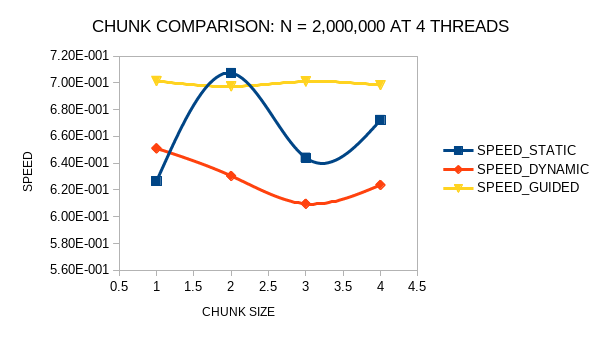
\includegraphics[width=150mm,height= 80mm]{chunk_2e6.png}\hspace*{\fill}
            \caption{Chunk size comparison for N = 2,000,000}
        \end{figure}

        \subsection{More Chunk Sizes}
        In order to investigate better, I tried to increase the chunk size for the extreme case: 2,000,000.  The results are as follow:

        \begin{figure}[H]
            \hfill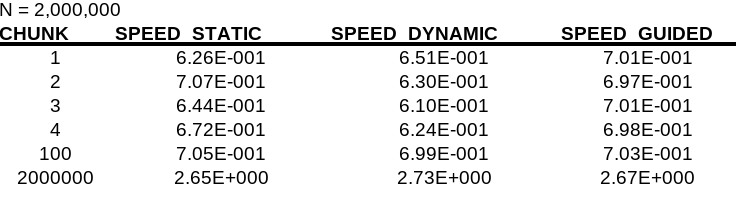
\includegraphics[width=150mm,height= 40mm]{chunkMAX.png}\hspace*{\fill}
        \end{figure}
        \noindent
        Clearly, increasing the chunk size does not really help. In fact, at the extreme when chunk size = problem size, then we have large overheads. 

        \newpage
        \section{Discussions}
        Firstly, for default schedulers, at higher NMAX, dynamic and guided schedulers perform better than static scheduler. In fact, from Figures 1 to 4, we can see that the static scheduler is always the one that does not perform well compare to dynamics and guided.  The reason for this is that the static scheduler does not perform well if individial iterations have widely different run times, which is the case for the Collantz conjecture. \newline

        \noindent
        Additionally, for a particular problem size, all default schedulers achieve speed up to to around 8 cores. At 16 cores, we ran into Blueshark's limitation of 12 cores per node.  We can see this very clearly when N = 20,000; the recorded speedups at 16 cores are significantly lower than our results at 8 cores. 

        \noindent
        Secondly, the max speedup that I can get using Blueshark is using NMAX = 20,000 and using the default guided schedule with 8 cores.  With this configuration, I got a speedup of around 9.13, according to figures and result tables in Section 3.2. This is actually better than theoretical speedup for 8 cores. In contrast, 16 cores do not give very good results and the reason might be that Blueshark is limited by 12 cores per node.  \newline

        \noindent
        Finally, the chunk size also plays a role in this assignment.  Surprisingly, higher chunk size tends to benefit the static scheduler.  We can see this in Figure 5 to 8. Unfortunately, we will not get any speedup if we keep increase the chunk size. Section 3.4 shows this for NMAX = 2,000,000; at the extreme when chunk size = problem size, we have large overheads.  At chunk size of 100, we did not see any improvements from the smaller chunk sizes. 

        \newpage
        \section{Code}

        \begin{lstlisting}
    PROGRAM test

    use omp_lib 
    IMPLICIT NONE
    INTEGER*8 :: n,iterNMAX,j,highN, GLOBAL_MAX 
    INTEGER*8 :: maxHOTPO 

    INTEGER*8 :: nstart, nend 

    INTEGER :: num_threads 
    DOUBLE PRECISION :: tstart, tend, t_elapse
    
    GLOBAL_MAX = 0 
    maxHOTPO = 1e8

    num_threads = 4 
    call OMP_SET_NUM_THREADS(num_threads)

    nstart = 1
    nend = 200000 

    tstart = OMP_GET_WTIME()

    !$OMP PARALLEL DO SCHEDULE(GUIDED,4) PRIVATE(iterNMAX,j,n,highN)&
    !$OMP SHARED(maxHOTPO,nstart,nend) REDUCTION(max:GLOBAL_MAX) 
    DO iterNMAX = nstart,nend
        n = iterNMAX
        highN = 0
        DO j = 1,maxHOTPO        
            !! local max 
            IF(n > highN) THEN 
                highN = n 
            END IF 

            
            call hotpo(n)

            IF (n == 1) THEN 
                EXIT 
            END IF

            !! global max 
            IF(highN > GLOBAL_MAX) THEN 
                GLOBAL_MAX = highN
            END IF

        END DO 

    END DO
    !$OMP END PARALLEL DO 
    

    tend = OMP_GET_WTIME() 

    t_elapse = tend - tstart 


    WRITE(*,*) ""
    WRITE(*,*) "PROBLEM SIZE: ", nend
    WRITE(*,*) "RUNNING WITH ", num_threads, " CORES"
    WRITE(*,*) "Time taken :",t_elapse  
    WRITE(*,*) "GLOBAL MAX = ", GLOBAL_MAX



END PROGRAM test 



SUBROUTINE hotpo(ndum)
    IMPLICIT NONE
    INTEGER*8, INTENT(INOUT) :: ndum

    IF (mod(ndum,2) == 0) THEN
        ndum = ndum / 2 
    ELSE
        ndum = (3 * ndum ) + 1
    END IF

    IF (ndum == 1) THEN
        ndum=1
    END IF

END SUBROUTINE hotpo 

            
        \end{lstlisting}




\end{document}